This chapter describes the benchmarking program, its input parameters, and the specification of the machines, that were used for the performance evaluation. Additionally, the results of the benchmark runs are analyzed (the results itself are presented in Appendix B) .

\section{Benchmark}

The performance evaluations is done with the benchmarking program. For each tested data structure (presented in \Cref{ch:numdb} and \Cref{ch:alt}), the benchmark runs for a specified amount of time. Then the throughput (operations per second) is calculated as the total count of iterations divided by the total time.

Instead of separately measuring the performance of every basic operation (\findop, \insertop, \removeop), the overall numeric database performance is evaluated. The numeric database retrieval operation consists of either lookup (in case the item with the specified key is in the database) or lookup, user function invocation, item removal and item insertion. The user function is much slower than the database operations. Therefore, the most effective numerical database is the one that calls the user function as rarely as possible.

The recursive computation of the $N$th Fibonacci number is chosen as the user function. The algorithm implementation is trivia and, having the exponential time complexity, it is extremely inefficient. This is the advantage from the perspective of the benchmark as its task is to simulate a very computational-heavy function. What is more, the time it takes to compute the function can be easily adjusted by the function argument.

\pagebreak

Generally, cache systems perform well only on skewed inputs, when there is a small subset of items that are accessed most of the time while other items are accessed much less often. In this benchmark, a numerical database is tested with a random input sequence that has normal distribution of values. The parameters of the distribution are as follows:
\begin{description}
\item[Mean $u$] equals zero. The data structures presented in this library are agnostic to the particular argument values and their performance is only affected by the frequency of items in the input sequence. So $u$ can be any number. Zero is any number.

\item [Standard deviation $\sigma$] is derived from $Area{\mhyphen}under{\mhyphen}curve$ parameter and the available memory. $Capacity$ is calculated as the available memory divided by the size of a single item. $Area{\mhyphen}under{\mhyphen}curve$ is a value from the interval $(0,1)$. It defines the ratio of accesses to the $Capacity$ most valuable items to the total count of accesses. With given $Capacity$ and $Area{\mhyphen}under{\mhyphen}curve$, $\sigma$ is calculated as follows:
\begin{equation}
 \sigma = \frac{Capacity}{2 \times Quantile(0.5 + \frac{Area{\mhyphen}under{\mhyphen}curve}{2})}
 \end{equation}
\end{description}

\section{Benchmark Parameters}
The benchmark has several input parameters:
\begin{description}
\item [minval, maxval]-- the range of values the Fibonacci function is called with. It is defined as a range to simulate functions which execution time depends on its arguments.
\item [available memory]-- the maximum amount of memory the numerical database uses.
\item [thread count]-- relevant for concurrent numerical databases. Sets the number of  threads to run in parallel.
\item[mean changing rate]-- adjusts the rate at which the mean of the distribution is changed. If larger than zero, it simulates input sequences with non-static distribution. It is measured in the \emph{delta-per-iteration} units~-- its value is added to the mean at every iteration, e.g. if the rate is $^1/_{100}$, than after 1000 iteration the mean will move by 10.
\item[area-under-curve]-- the parameter that affects the standard deviation of the distribution.
\end{description}

\section{Analysis of the Sequential Containers}

\label{sec:secanalysis}

The performance evaluation of the sequential containers has been done on the following machine:

\begin{description}
    \item [CPU] Intel\textsuperscript{\textregistered{}} Core\textsuperscript{\texttrademark{}} i5-6200U
    2.30GHz (2.80 GHz\footnote{with Intel\textsuperscript{\textregistered{}} Turbo Boost Technology})$ \times$ 2 cores
    \item [Memory] 8 GB DDR3 1600 MHz
    \item [OS] Linux\textsuperscript{\textregistered{}} Ubuntu\textsuperscript{\textregistered{}} 16.04 LTS 64-bit
    \item [Compiler] GCC 5.4, compilation flags: \texttt{-O3 -std=c++14}
    \end{description}

In this chapter there are several graphs (\Cref{f1}, \Cref{f2}, \Cref{f3}), that visualises data presented in \Cref{ch:bresult}. The graphs do not include all the data from the tables, e.g. there is no graph for LRU and LFU based numerical databases; only the most representative candidates have been chosen. The outcomes have confirmed some assumptions, stated in the previous chapters, while refuted others.

The weighted search tree proved to be the most effective container for the numerical database. However, no concurrent WST implementation is known, so its usage is limited to the sequential environment.

The combination of the hash table and the binary heap performs about 10\% slower than WST. However, its advantage over WST is the simpler structure, that made it possible to develop the concurrent version of this container, called \cndcname.

The benchmark proved splay tree inefficiency. It is outperformed by WST and the hash table on all workloads. Therefore it is not recommended to use it for a numerical database.

\emph{Least-recently-used} and \emph{Least-frequently-used} eviction policies do not achieve the same performance as the policy, based on the binary heap. Possibly, because they do not rely on the initial item priority, thus give no preference to items that are rarely accessed  but took long to be calculated and due to that must be kept in the database.

\emph{Priority aging} does not show any advantage over the static priority. However, further studies and tests are required here, as the benchmark does not simulate the worst-case input for the static priority scheme.

\begin{figure}[h]
\centering
    \label{f1}
    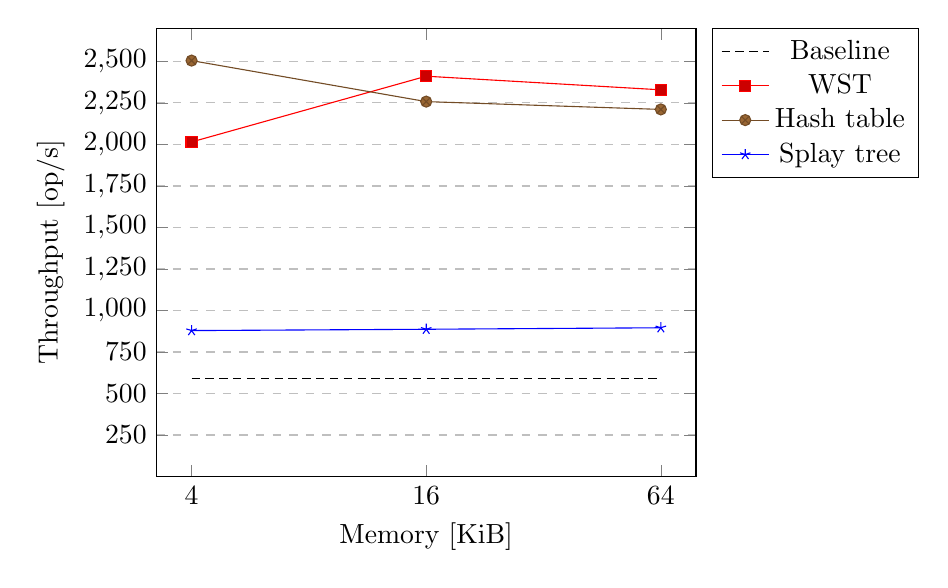
\begin{tikzpicture}
      \begin{axis}[
        legend pos=outer north east,
        xlabel = Memory {[KiB]},
        ylabel = Throughput {[op/s]},
        xmin = 0.85, xmax = 3.15,
        xtick={1,2,3},
        xticklabels={4, 16, 64},
        ymin = 0, ymax = 2700,
        ytick={250, 500, 750, 1000, 1250, 1500, 1750, 2000, 2250, 2500},
        ymajorgrids=true,
        grid style=dashed,
      ]
        \addplot+[densely dashed, color=black, mark = no] coordinates{(1, 588)(2, 588)(3, 588)};
        \addplot coordinates{(1, 2015)(2, 2411)(3, 2329)};
        \addplot coordinates{(1, 2505)(2, 2258)(3, 2211)};
        \addplot+[color=blue] coordinates{(1, 879)(2, 887)(3, 896)};
        \legend{Baseline,WST,Hash table,Splay tree}
      \end{axis}
      \end{tikzpicture}
\caption{Sequential containers comparison (variable memory size)}
\end{figure}


\begin{figure}
\centering
    \label{f2}
    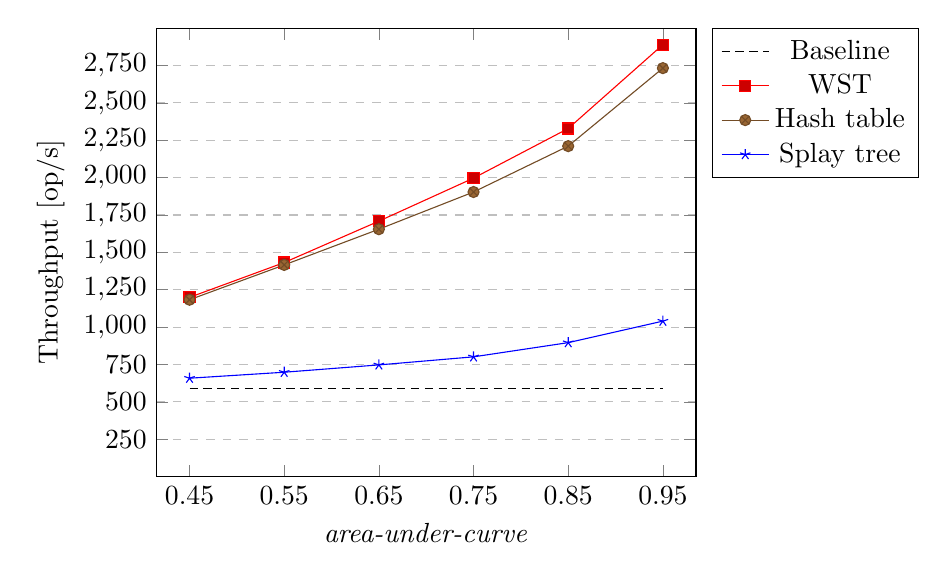
\begin{tikzpicture}
      \begin{axis}[
        legend pos=outer north east,
        xlabel = \emph{area-under-curve},
        ylabel = Throughput {[op/s]},
        xmin = 0.65, xmax = 6.35,
        xtick={1,2,3,4,5,6},
        xticklabels={0.45, 0.55, 0.65, 0.75, 0.85, 0.95},
        ymin = 0, ymax = 3000,
        ytick={250, 500, 750, 1000, 1250, 1500, 1750, 2000, 2250, 2500, 2750},
        ymajorgrids=true,
        grid style=dashed,
      ]
        \addplot+[densely dashed, color=black, mark = no] coordinates{(1, 588)(2, 588)(3, 588)(4, 588)(5,588)(6,588)};
        \addplot coordinates{(1, 1199)(2, 1432)(3, 1709)(4, 1997)(5,2329)(6,2890)};
        \addplot coordinates{(1, 1183)(2, 1416)(3, 1655)(4, 1904)(5,2211)(6,2733)};
        \addplot+[color=blue] coordinates{(1, 658)(2, 698)(3, 747)(4, 801)(5,896)(6,1040)};
        \legend{Baseline,WST,Hash table,Splay tree}
      \end{axis}
    \end{tikzpicture}
\caption{Sequential containers comparison (variable \emph{area-under-curve} value)}
\end{figure}


\begin{figure}[!t]
\centering
    \label{f3}
    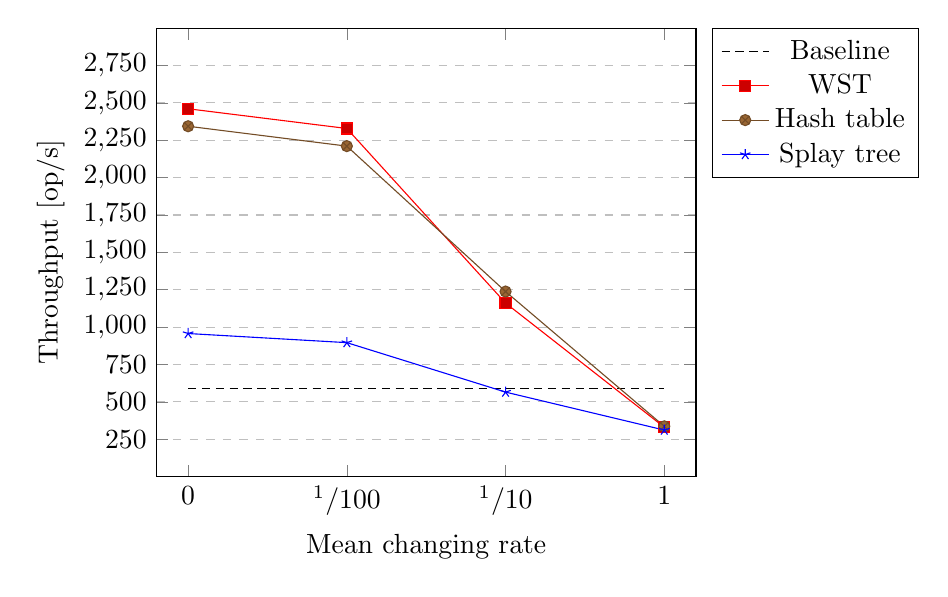
\begin{tikzpicture}
          \begin{axis}[
            legend pos=outer north east,
            xlabel = Mean changing rate,
            ylabel = Throughput {[op/s]},
            xmin = 0.80, xmax = 4.20,
            xtick={1,2,3,4},
            xticklabels={0, $^1/{100}$, $^1/{10}$, 1},
            ymin = 0, ymax = 3000,
            ytick={250, 500, 750, 1000, 1250, 1500, 1750, 2000, 2250, 2500, 2750},
            ymajorgrids=true,
            grid style=dashed,
          ]
            \addplot+[densely dashed, color=black, mark = no] coordinates{(1, 588)(2, 588)(3, 588)(4, 588)};
            \addplot coordinates{(1, 2461)(2, 2329)(3, 1161)(4, 330)};
            \addplot coordinates{(1, 2344)(2, 2211)(3, 1238)(4, 336)};
            \addplot+[color=blue] coordinates{(1, 957)(2, 896)(3, 565)(4, 311)};
            \legend{Baseline,WST,Hash table,Splay tree}
          \end{axis}
        \end{tikzpicture}
\caption{Sequential containers comparison (variable mean changing rate)}
\end{figure}


\section{Analysis of the Concurrent Containers}

\label{sec:conanalysis}

The performance evaluation of the concurrent containers has been performed on the following machine:

\begin{description}
    \item [CPU] Intel\textsuperscript{\textregistered{}} Xeon\textsuperscript{\textregistered{}} E5-2650 v4
    2.20GHz (2.90 GHz\footnote{with Intel\textsuperscript{\textregistered{}} Turbo Boost Technology}) $ \times $ 2 sockets $ \times $ 12 cores
    \item [Memory] 256 GB DDR4 2400 MHz
    \item [OS] Linux\textsuperscript{\textregistered{}} Ubuntu\textsuperscript{\textregistered{}} 16.04 LTS 64-bit
    \item [Compiler] GCC 5.4, compilation flags: \texttt{-O3 -std=c++14}
    \end{description}

Same as with the sequential containers, the complete benchmark data is presented in \Cref{ch:bresult}. \Cref{f4} shows the performance difference between the tested concurrent containers. \Cref{f5} demonstrates their scalability~-- the relative per-thread performance with increasing number of threads. For example, the graph shows that with 24 threads running simultaneously, the performance of one thread in \cndcname is 30\% lower than that in the single-threaded test.

As expected, the coarse-grained locking approach yields the very ineffective container. The observation that with 2 threads the performance is two times lower compared to the single-threaded test (note, the total, not the per-thread performance) can be explained by the high contantion on the single mutex. The process of locking/unlocking an open mutex is quite fast operation, but locking the already locked mutex implies, that the thread will be suspended and then resumed. This is quite heavy and complex operation from the perspective of an operational system.

The binning approach performs better than the previous one. However, \Cref{f5} clearly shows, that it does not scale very good for the bigger number of threads~-- at 24 threads, per-thread performance is only 10\% as high as the maximum.

\cndcname shows excellent scalability, even with 24 threads. The poor per-thread performance is rather explained by the huge memory overhead per item than by computational complexity~-- in addition to the overhead, introduced by the data structure itself, synchronization adds at least 60 bytes for each item. The further studies should be directed at lowering this overhead. For example, some synchronization can be performed in the lock-free fashion with no mutexes involved.

\begin{figure}
\centering
    \label{f4}
    \begin{tikzpicture}
          \begin{axis}[
            legend pos=outer north east,
            xlabel = Thread count,
            ylabel = Throughput {[op/s]},
            ylabel shift = 0.5 pt,
            xmin = 0, xmax = 26,
            xtick={1, 2, 4, 8, 16, 24},
            ymin = 0, ymax = 1400,
            ytick={100, 200, 300, 400, 500, 600, 700, 800, 900, 1000, 1100, 1200, 1300},
            yticklabels={1000, 2000, 3000, 4000, 5000, 6000, 7000, 8000, 9000, 10000, 11000, 12000, 13000},
            ymajorgrids=true,
            grid style=dashed,
          ]
            \addplot coordinates{(1, 73.4)(2, 152.4)(4, 298.4)(8, 512.0)(16, 904.0)(24, 1292.0)};
            \addplot coordinates{(1, 234)(2, 123)(4, 120)(8, 127)(16, 124)(24, 127)};
            \addplot+[mark = triangle, mark options=solid]
                     coordinates{(1, 223)(2, 279)(4, 332)(8, 379)(16, 525)(24, 636)};

            \legend{\cndcname, Coarse + WST, Binning + WST}
          \end{axis}
        \end{tikzpicture}
\caption{Concurrent containers comparison (variable thread count)}
\end{figure}

\begin{figure}
\centering
    \label{f5}
    \begin{tikzpicture}
          \begin{axis}[
            legend pos=outer north east,
            xlabel = Thread count,
            ylabel = Relative performance per thread,
            xmin = 0, xmax = 26,
            xtick={1, 2, 4, 8, 16, 24},
            ymin = 0, ymax = 1.1,
            ytick={0.1, 0.2, 0.3, 0.4, 0.5, 0.6, 0.7, 0.8, 0.9, 1},
            ymajorgrids=true,
            grid style=dashed]
              \addplot coordinates{(1, 1)(2, 1.03)(4, 0.97)(8, 0.87)(16, 0.77)(24, 0.70)};
              \addplot coordinates{(1, 1)(2, 0.26)(4, 0.127)(8, 0.067)(16, 0.033)(24, 0.02)};
              \addplot+[mark = triangle, mark options=solid]
                       coordinates{(1, 1)(2, 0.626)(4, 0.37)(8, 0.212)(16, 0.147)(24, 0.119)};
              \legend{\cndcname, Coarse + WST, Binning + WST}
          \end{axis}
    \end{tikzpicture}
    \caption{Concurrent containers scalability comparison}
\end{figure}
